\section{Symmetry reduction for dynamical systems}
\label{sec:symReduce}

In a dynamical system with discrete or continuous symmetries,
points in the \statesp\ which are related to each
other by symmetry operation should be treated as a group.
Each member of this group has the same dynamical properties, so
we say that they are dynamically equivalent.
It is a good practice to choose a single representative in each
group and study the dynamics of this representative point instead.
This treatment is called \emph{symmetry reduction}. The
new \statesp\ that this representative point lives in is called
the \emph{(symmetry-)reduced \statesp}
After it was invented, symmetry reduction becomes
extremely successful for simplifying the analysis
of a dynamical system with symmetries. In this section,
we will discuss symmetry reduction techniques and study
the tangent dynamics in the reduced \statesp.

\subsection{Continuous symmetry reduction}
\label{sec:cred}

We use the same setup as in \refsect{sec:covVecs} and copy a
few equations here for convenience.
The content of this subsection is based on the materials in\rf{DasBuch}.
Let $ \dot{\ssp} = \vel(\ssp) \,,\ssp(x, t) \in \reals^n$  define a flow.
Usually we omit the dependence on coordinates, and write $\ssp(t)$.
Denote the evolution semigroup of this flow by $\ssp(t)=\flow{t}{\ssp_0}$.
We say that this flow
is equivariant under a continuous symmetry group $\Group$ if
\begin{equation}
  \label{eq:equivariant}
   \LieEl \vel(\ssp) =  \vel(\LieEl \ssp) \,,\quad
   \LieEl \flow{t}{\ssp} = \flow{t}{\LieEl \ssp}
   \quad \text{for any} \quad  \LieEl \in \Group
   \,.
\end{equation}
The two equations above are equivalent.
In practical applications, $\Group$ is always a Lie group.
Basically,
\refeq{eq:equivariant} means that if two starting states, which
are related to each other by a group operation, evolve for the same period of
time, then
the end states are related by the same group operation.

Now we introduce the terminology that will be used in the later discussion.
In is often more convenient to write the Lie group
$\Group$ in its exponential form
\begin{equation}
  \LieEl(\gSpace)=e^{\gSpace \,\cdot\, \Lg }
  \,,\qquad
  \gSpace \cdot \Lg  = \sum_{a=1}^s \gSpace_a \Lg_a
  \,,
  \label{eq:Lie}
\end{equation}
where $\Lg_a$, $a=1, 2\cdots, s$
are the \emph{generators} of $\Group$, and $\gSpace_a$ are
the parameters of this group.  Dot product refers to a sum over
generators in this section.
Generators of a real representation are antisymmetric:
\begin{equation}
  \label{eq:Tanti}
  \transp{\Lg_a} = - \Lg_a
  \,,
\end{equation}
where $\transp{\Lg_a}$ denotes the transpose of $\Lg_a$.
Let's work out a simple example. The
translation group $\{ g : g(x_0)\ssp(x, t) = \ssp(x+x_0, t) \}$
is denoted as $g(x_0) = \exp(x_0 \frac{\partial}{\partial x})$. Here,
$\frac{\partial}{\partial x}$ is the only generator and
$x_0$ is the parameter. Furthermore, we assume that the generators
of $\LieEl(\gSpace)$ commute with each other: $\Lg_a\Lg_b = \Lg_b\Lg_a$.

We define the \emph{group orbit} of a point $\ssp$ as
\begin{equation}
  \mathrm{Orb}(\ssp) = \{\LieEl\,\ssp : \LieEl \in {\Group}\}
  \,.
  \label{eq:orb}
\end{equation}
A group orbit is an $s$\dmn\ manifold, but it is
not a real orbit. It is a collection of all
dynamically equivalent points.
The \emph{group tangent} of state $\ssp$ is defined as
\begin{equation}
  \groupTan_a(\ssp)_{i}= (\Lg_a){}_{ij} \ssp_j
  \,,
  \label{eq:gTan}
\end{equation}
which is basically a matrix-vector product.
Note, \refeq{eq:equivariant} says that the flow equation is
equivariant under $\Group$, but it does not mean that
any orbit in the \statesp\ possesses all symmetries in $G$.
Now we define several important invariant structures.

\paragraph{\Eqv} $\ssp(\zeit) = \ssp(0)$. Namely, $\vel(\ssp) = 0$.

\paragraph{\Reqv} A state point $\ssp(x, t)$
is a \reqv\ if
\begin{equation}
  \ssp(\zeit) = \LieEl(\zeit \, \velRel) \, \ssp(0)
  \,=\, e^{\zeit \, \velRel \cdot \Lg} \ssp(0)
  \,,
  \label{eq:req}
\end{equation}
where $c$ is a constant. Definition \refeq{eq:req} is equivalent to
$\vel(\ssp) = \velRel \cdot \groupTan(\ssp)$. A \reqv\ is
very similar to an \eqv\ except for a constant drifting in the
group direction.

\paragraph{\Po}  $\ssp(\period{p}) = \ssp(0)$. $\period{p}$ is the
period.

\paragraph{\Rpo} Similar to \po s,
if a state returns to its initial state except for
a group translation after a center time, then we say that
this point is on a \rpo.
\begin{equation}
  \ssp_p (0) = \LieEl_p \ssp_p (\period{p} )
  \,,
  \label{eq:rpo}
\end{equation}
where $\period{p}$ is the period. $\LieEl_p = \LieEl(\gSpace_p)$
takes the end state to the initial state. We use subscript $p$ to
indicate that the variable belongs to a \po\ or \rpo.

With the above setup, we illustrate how to use
\emph{slice} to reduce continuous symmetries.
The idea is similar to a Poincar\'e section.
We define a slice that cuts every group orbit only once, so that we
can use this
intersection point as the representative of the whole group orbit.
The simplest slice is a flat hypersurface that is normal to the
group tangent of a pre-specified point $\slicep$:
\begin{equation}
  \braket{\sspRed - \slicep}{\sliceTan{a}} = \braket{\sspRed}{\sliceTan{a}} = 0
  \,,\quad
  \sliceTan{a} = \groupTan_a(\slicep) = \Lg_a \, \slicep
  \,,\quad
  \text{for} \quad a = 1, 2, \cdots, s
  \,.
  \label{eq:slice}
\end{equation}
Here, we use a bra-ket notation for the inner product of two
real vectors in $\mathbb{R}^n$,
\[
  \braket{u}{w} = \transp{u} w = \sum_{i=1}^n u_i w_i
  \,.
\]
A hat on a state indicates that it is a state in the symmetry-reduced \statesp.
Definition \refeq{eq:slice} has used
$\braket{\slicep}{\sliceTan{a}} = \braket{\slicep}{\Lg_a \, \slicep} = 0$
which is the result of the antisymmetry of $\Lg_a$ \refeq{eq:Tanti}.
Now, symmetry reduction turns out to be a process of finding
a specific group element $\LieEl(\gSpace)$ that transforms each state
$\ssp$ into the slice.
\begin{equation}
  \sspRed = \LieEl^{-1}(\gSpace) \, \ssp
  \,.
  \label{eq:slice2}
\end{equation}
$\sspRed$ is the state on the slice that represents $\ssp$ and the whole group orbit
of $\ssp$. Note, it usually requires different group parameter $\gSpace$ for
different states in \refeq{eq:slice2}.
Equivalently, we can recover the state in the full \statesp\ by
the state in the symmetry-reduced \statesp\ and the group parameter $\gSpace$,
\begin{equation}
  \label{eq:slice3}
  \ssp = \LieEl(\gSpace) \, \sspRed
  \,.
\end{equation}

The symmetry reduction process described above is called the \emph{post-processing}
method. That is, we need to know the trajectory beforehand in order to reduce
it into the slice. However, many a time, it is more efficient to integrate
the system in the slice directly. This posts a question of what the dynamics is
like in the slice. Let us start from finding the reduced velocity in the slice.
Take the time derivative of both sides of \refeq{eq:slice3},
$ \vel(\LieEl\sspRed) = \vel(\ssp) = \dot{\LieEl}\sspRed + \LieEl\velRed $.
Rewrite it with $\velRed = \LieEl^{-1} \vel(\LieEl \, \sspRed)
- \LieEl^{-1} \dot{\LieEl} \, \sspRed$ and the equivariance condition
\refeq{eq:equivariant} leads to
$\velRed = \vel - \LieEl^{-1} \dot{\LieEl} \, \sspRed $.
Also,  by \refeq{eq:Lie} and the definition of the group tangent \refeq{eq:gTan}, we
get
\[
  \LieEl^{-1} \dot{\LieEl}\, \sspRed  = \sum_{a=1}^s \dot{\gSpace}_a(\sspRed)
  \, \Lg_a \sspRed =
  \sum_{a=1}^s \dot{\gSpace}_a(\sspRed) \groupTan_a(\sspRed)
  \,.
\]
So the velocity in the slice is given as
\begin{equation}
  \velRed(\sspRed)
  = \vel(\sspRed)
  \,-\, \sum_{a=1}^s \dot{\gSpace}_a(\sspRed) \groupTan_a(\sspRed)
  \label{eq:svel}
\end{equation}
The dynamics of $\gSpace_a(\sspRed)$
is governed by the slice. Taking the time derivative of the slice condition
\refeq{eq:slice} and substituting \refeq{eq:svel}, we get
\[
  \braket{\sliceTan{a}}{\velRed(\sspRed)} =
  \braket{\sliceTan{a}} {\vel(\sspRed)} -
  \sum_{b=1}^s \braket{\sliceTan{a}}{\groupTan_b(\sspRed)} \, \dot{\gSpace}_b
  = 0
  \,, \quad
  \text{for} \quad a = 1, 2,\cdots, s
  \,.
\]
This defines $s$ linear equations with total $s$ unknowns. Define the
coefficient matrix as $L$ whose element is
\begin{equation}
  \label{eq:phiL}
  L(\sspRed)_{ab} =  \braket{\sliceTan{a}}{\groupTan_b(\sspRed)}
  \,,
\end{equation}
then we can solve the equation for $\dot{\gSpace}_a(\sspRed)$.
In summary, the dynamics in the slice is governed by
\begin{eqnarray}
  \velRed(\sspRed)
  & = & \vel(\sspRed)
        \,-\, \sum_{a=1}^s \dot{\gSpace}_a(\sspRed) \groupTan_a(\sspRed)
        \,,\qquad\quad \sspRed \in \pSRed
        \label{EqMotMFrame0} \\
  \dot{\gSpace}_a(\sspRed)
  & = &  \sum_{b=1}^{s}(L^{-1})_{ab} \braket{\sliceTan{b}}{\vel(\sspRed)}
        \,,\qquad\quad a = 1, 2, \cdots, s
        \label{MFdtheta0}
        \,.
\end{eqnarray}
The above in-slice dynamics fails when $L$ is singular. One obvious cause of
failure is a situation where some $\sliceTan{a}$ are parallel. So when
choosing the template points for defining the slice, we need to guarantee
that $\sliceTan{a}$, $a=1, 2, \cdots, s$ are not parallel. Under this
assumption, a slice fails only when the in-\slice\ state $\sspRed$
makes \refeq{eq:phiL} singular. The set of these points defines the
\emph{border} of the slice.

When the group has only one parameter $\gSpace$, then matrix $L$ is
a scalar and the above formula can be simplified as
\bea
\velRed(\sspRed) &=& \vel(\sspRed)
                    \,-\, \dot{\gSpace}(\sspRed) \groupTan(\sspRed)
    \,,\qquad\quad \sspRed \in \pSRed
\label{EqMotMFrame}
\\
\dot{\gSpace}(\sspRed) &=&
                            {\braket{\vel(\sspRed)}{\sliceTan{}}}/
                            {\braket{\groupTan(\sspRed)}{\sliceTan{}}}
\label{MFdtheta}
\,.
\eea


\subsection{Tangent dynamics in the slice}
\label{sect:tang}

Equations \refeq{EqMotMFrame0}\refeq{MFdtheta0} or
\refeq{EqMotMFrame}\refeq{MFdtheta} describe the dynamics
in the slice, by which we can obtain the whole in-slice
trajectory given a starting in-slice state. However, sometimes
we not only desire the in-slice orbit but also the
tangent dynamics in the slice. More precisely,
formulas \refeq{eq:stab} and \refeq{eq:tangentDynamics}
describe the tangent dynamics in the full \statesp. What are
the corresponding formulas in the slice? What is the relation
between \JacobianM\ in the slice and that in the full \statesp?
This subsection is devoted to answering
these questions. For simplicity, in the following, we assume
that the continuous group has only one parameter, \ie, $s=1$ in
\refeq{eq:Lie}. Nevertheless, the technique described
below can be easily extended to symmetries with more than one
group parameter.

\begin{figure}[h]
  \centering
  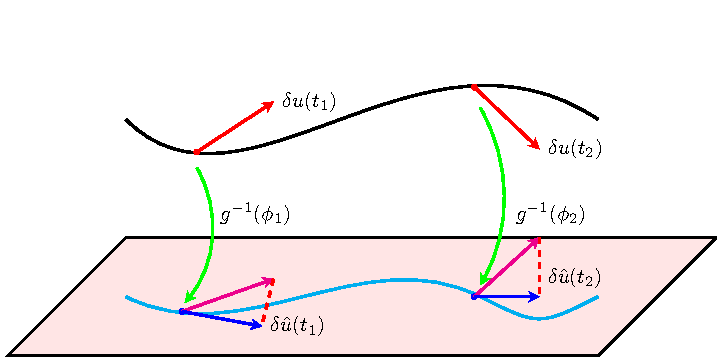
\includegraphics[width=0.9\linewidth]{jacobian_full_slice}
  \caption[Jacobian in the slice]{
    The relation between deformations in
    the full {\statesp} and in the \slice.
    The pink plane is the slice. The black curve is a trajectory in the {\statesp}.
    The cyan curve is the corresponding trajectory in the {\slice}.
    Infinitesimal deformation $\delta \ssp(t_1)$ at time $t_1$
    is transported to $\delta \ssp(t_2)$ at time $t_2$.
    $\delta \sspRed(t_1)$ and $\delta \sspRed(t_2)$ are the in-slice
    correspondents.
  }
  \label{fig:jacobian_full_slice}
\end{figure}

First, we investigate how infinitesimal deformation is
transformed into the slice from the full \statesp.
We start from the \slice\ condition \refeq{eq:slice}.
Infinitesimal deformation $\delta \sspRed$ at $\sspRed$
should be confined to the \slice\ too, so we have a constraint
\begin{equation}
  \braket{\delta \sspRed}{\sliceTan{}}=0
  \,.
  \label{eq:constraint_dx}
\end{equation}
Here, the subscript of $\sliceTan{}$ is omitted because we assume
that there
is only one group parameter.
Taking the derivative of \refeq{eq:slice3} we get
$ \delta \ssp = \delta \LieEl(\gSpace) \sspRed + \LieEl(\gSpace)
\delta \sspRed $ which is equivalent to
\[
  \delta \sspRed=-\Lg \sspRed\delta \gSpace + \LieEl(\gSpace)^{-1}\delta\ssp
  \,.
\]
Substituting it into \refeq{eq:constraint_dx},
we get
$\braket{-\mathbf{T}\sspRed\delta \gSpace + \LieEl(\gSpace)^{-1}
\delta\ssp}{t'}=0$
which is
\begin{equation}
  \label{eq:delta_theta}
  \delta \gSpace=
  \frac{\braket{\sliceTan{}}{\LieEl(\gSpace)^{-1}\delta\ssp}}
  {\braket{\groupTan(\sspRed)}{\sliceTan{}}}
\,.
\end{equation}
Now  $\delta \sspRed$, the infinitesimal deformation in the \slice, can be
expressed by the deformation in the full {\statesp} $\delta\ssp$:
\begin{equation*}
  \ket{\delta \sspRed}
  =
  -\frac{\braket{\sliceTan{}}{\LieEl(\gSpace)^{-1}\delta\ssp}}
  {\braket{\groupTan(\sspRed)}{\sliceTan{}}}
  \ket{\groupTan(\sspRed)}
  + \LieEl(\gSpace)^{-1} \ket{\delta \ssp}
  \,,
\end{equation*}
that is,
\beq
\label{eq:variation_full_slice}
\ket{\delta \sspRed} =
\left(\matId-\frac{\ket{\groupTan(\sspRed)}\bra{\sliceTan{}}}
  {\braket{\groupTan(\sspRed)}{\sliceTan{}}} \right)
\LieEl(\gSpace)^{-1}\ket{\delta \ssp}
:=
h(\sspRed)\LieEl(\gSpace)^{-1}\ket{\delta \ssp}
\eeq
The physical interpretation of \refeq{eq:variation_full_slice} is manifest.
Infinitesimal deformation $\delta \ssp$ at $\ssp$ in the full {\statesp} is
first transformed to point $\sspRed$ by $\LieEl(\gSpace)^{-1}$ and then
projected into the {\slice} by $h(\sspRed)$ illustrated in
\reffig{fig:jacobian_full_slice}.
The matrix
\beq
\pMat(\sspRed)=
    \matId-\frac{\ket{\groupTan(\sspRed)}\bra{\sliceTan{}}}
    {\braket{\groupTan(\sspRed)}{\sliceTan{}}}
%\,.
\ee{projFullToSlice}
projects infinitesimal deformation in the full {\statesp} into the {\slice}.
It is singular and has the following properties.
\begin{itemize}
\item $h(\sspRed)\ket{\groupTan(\sspRed)}=0$ :
  any infinitesimal deformation along the group tangent direction
  at $\sspRed$ in the full {\statesp} will disappear after projection.

\item $\bra{\sliceTan{}}h(\sspRed)=0$ : any vector projected into the {\slice} will be
  perpendicular to the group tangent of the template point as expected. This
  property and the above one both prove that matrix $h(\sspRed)$ is not full-rank.

\item In-slice velocity \refeq{EqMotMFrame} turns out to be
  \[
    \velRed(\sspRed)= \vel(\sspRed)
    -\frac{\braket{\vel(\sspRed)}{\sliceTan{}}}{\braket{\groupTan(\sspRed)}{\sliceTan{}}}
    \groupTan(\sspRed)=h(\sspRed)\vel(\sspRed)
    \,.
  \]
  The velocity field is transformed by matrix $h(\sspRed)$.
\end{itemize}

Since projection matrix \refeq{projFullToSlice} is singular,
the projection
reduces the dimension of the system by one.
However, \refeq{projFullToSlice} is still expressed in
the full {\statesp}.
In practice,
we desire to work in a lower\dmn\ system after quotienting out
the continuous symmetry.
Now let's decrease the dimension of all matrices and
vectors in the {\slice} by one explicitly.
Denote
\[
  \pMat(\sspRed)=
  \begin{bmatrix}
    h_{1} \\
    h_{2} \\
    \vdots \\
    h_{n}
  \end{bmatrix}
  \,.
\]
Each $h_{i}$ is a row vector and $n$ is the dimension of the full {\statesp}.
From the second property of $h(\sspRed)$ we know that $h_{i}$ are linear
dependent: $\sliceTan{1}h_{1}+\sliceTan{2}h_{2}+\cdots +\sliceTan{n}h_{n}=0$.
Here $\sliceTan{i}$ are
components of vector $\sliceTan{}$.
Assume $t'_{\xi}\neq 0$, then
\[
h_{\xi}=\sum_{i=1,i\neq \xi}^{n}-\frac{\sliceTan{i}}{\sliceTan{\xi}}h_{i}
\]
so $h_{\xi}$ can be eliminated from $\pMat(\sspRed)$:
\[
  \pMat(\sspRed)=
  \underbrace{
    \begin{bmatrix}
      1 & & & & \\
      & 1 & & & \\
      & & \ddots & & \\
      -\frac{\sliceTan{1}}{\sliceTan{\xi}} &
      -\frac{\sliceTan{2}}{\sliceTan{\xi}} & & \cdots &
      -\frac{\sliceTan{n}}{\sliceTan{\xi}} \\
      & & & \ddots  & \\
      & & & & 1 \\
    \end{bmatrix}
  }_{n\times (n-1)}
  \underbrace{
    \begin{bmatrix}
      h_{1} \\
      \vdots \\
      h_{\xi-1} \\
      h_{\xi+1} \\
      \vdots \\
      h_{n} \\
    \end{bmatrix}
  }_{(n-1)\times n}
  := P'\pMatM(\sspRed)
  \,.
\]
The above expression is the {rank factorization}
of $h(\sspRed)$ with $\pMatM(\sspRed)$ a full-rank matrix.
The superscript of the minus sign indicates that
the matrix (vector) is $(n-1)$\dmn.
Similarly, from the {\slice} condition $\braket{\sliceTan{}}{\sspRed}=0$,
we can reduce the dimension of a
point on the {\slice} by one
\[
  \sspRed=P'\sspRedM
\]
and also reduce the dimension of an infinitesimal deformation by one
\[
  \delta \sspRed=P'\delta \sspRedM
  \,.
\]
Here, $\sspRedM$ and
$\delta \sspRedM$ are both $(n-1)$\dmn\ vectors.
\[
  \sspRedM=\transp{[\sspRed_1, \cdots, \sspRed_{\xi-1}, \sspRed_{\xi+1}, \cdots, \sspRed_{n}]}
  \,, \quad
  \delta \sspRedM= \transp{[\delta \sspRed_1, \cdots, \delta \sspRed_{\xi-1},
    \delta \sspRed_{\xi+1}, \cdots, \delta \sspRed_{n}]}
  \,.
\]
Now relation \refeq{eq:variation_full_slice} can be rewritten as:
\begin{equation}
  \label{eq:projectionReduced}
  \ket{\delta \sspRedM} = \pMatM(\sspRed)\LieEl(\gSpace)^{-1}\ket{\delta \ssp}
\end{equation}
Note that the left side of the above equation
is an $(n-1)$\dmn\ vector while the right side $\ket{\delta \ssp}$
is an $n$\dmn\ vector and the $[(n-1)\times n]$ matrix $\pMatM(\sspRed)$
is the ``projection'' operator.

%%%%%%%%%%%%%%%%%%%%%%%%%%%%%%%%%%%%%%%%%%%%%%%%%%%%%%%%%%%%%%%%%%%%%%%%
\subsection{In-slice \JacobianM }
\label{sect:sliceJac}

Now let's turn to the transformation of the \JacobianM.
In \reffig{fig:jacobian_full_slice},
there is a trajectory from $\ssp(\zeit_1)$ to $\ssp(\zeit_2)$ in the full {\statesp}.
The corresponding transformed in-\slice\ trajectory is from $\sspRed(\zeit_1)$
to $\sspRed(\zeit_2)$.
Infinitesimal deformations in the full {\statesp} and in the
{\slice}  will be evolved by the
\JacobianM\ in the full {\statesp} and in the {\slice} respectively.
\begin{eqnarray}
  \jMps\delta \ssp(t_1) & = & \delta \ssp(t_2)
                              \label{eq:sliceJ}  \\
  \hat{\jMps}\delta \sspRedM(t_1) & = &\delta \sspRedM(t_2)
                                           \label{eq:sliceJ2}
                                           \,.
\end{eqnarray}
Here, $\jMps = J^{t_2 -t_1}(\ssp(t_1), \zeit_1)$ and
$\hat{\jMps} = J^{t_2 -t_1}(\sspRedM(t_1), \zeit_1)$.
For notation simplicity, we omit all parameters of \JacobianM\
if no confusion occurs.
Substituting \refeq{eq:projectionReduced} into \refeq{eq:sliceJ2},
we get
\[
  \hat{\jMps}  \pMatM(\sspRed(t_1)) \LieEl(\gSpace_1)^{-1} \delta\ssp(t_1)=
  \pMatM(\sspRed(t_2)) \LieEl(\gSpace_2)^{-1}\delta\ssp(t_2)
  =
  \pMatM(\sspRed(t_2)) \LieEl(\gSpace_2)^{-1}\jMps\delta\ssp(t_1)
  \,.
\]
The last step above has used relation \refeq{eq:sliceJ}.
This results in
\begin{equation}
  \label{eq:relation_jacobian1}
  \hat{\jMps}\pMatM
  (\sspRed(\zeit_1))\LieEl(\gSpace_1)^{-1}=
  \pMatM(\sspRed(\zeit_2))\LieEl(\gSpace_2)^{-1}\jMps
  \,.
\end{equation}
$\hat{\jMps}$ is an $[(n-1)\times (n-1)]$ matrix as we can easily see.
The geometrical meaning of relation \refeq{eq:relation_jacobian1} is obvious
in \reffig{fig:jacobian_full_slice}. On the left side, the
infinitesimal deformation $\delta \ssp(\zeit_1)$ at $\ssp(\zeit_1)$ is
transported to the slice first,
and then projected into the \slice, after which it is
evolved by $\hat{\jMps}$ to in-slice point
$\sspRed(\zeit_2)$. On the right side, the
infinitesimal deformation $\delta \ssp(\zeit_1)$ at $\ssp(\zeit_1)$ is evolved
first to $\ssp(\zeit_2)$
by $\jMps$, then transported to the slice, and finally projected
into the \slice.

By \refeq{eq:relation_jacobian1},
the relation between {\cLvs} in the full {\statesp} and in the {\slice}
can be obtained for
physically interesting invariant subsets: \eqva, \reqva, \po s, and
\rpo s.

\paragraph{In-slice stability matrix of an \eqv}
For an \eqv\ $\ssp(\zeit_1) = \ssp(\zeit_2) := \ssp_q$, we have
$\sspRed(\zeit_1)=\sspRed(\zeit_2) :=\sspRed_q$ and
$\gSpace_{1}=\gSpace_{2} := \gSpace_q$.
Formula \refeq{eq:relation_jacobian1} becomes
\begin{equation}
  \hat{\jMps}\pMatM
  (\sspRed_q)\LieEl(\gSpace_q)^{-1}=
  \pMatM(\sspRed_q)\LieEl(\gSpace_q)^{-1}\jMps
  \,.
  \label{eq:Jeqv0}
\end{equation}
Moreover, by \refeq{eq:tangentDynamics} we have $J=e^{(t_2-t_1)A}$
for \eqva, so \refeq{eq:Jeqv0} becomes
\begin{equation}
  \hat{A} \pMatM
  (\sspRed_q)\LieEl(\gSpace_q)^{-1}=
  \pMatM(\sspRed_q)\LieEl(\gSpace_q)^{-1}A
  \,,
  \label{eq:Jeqv1}
\end{equation}
where $\hat{A}$ is the in-slice stability matrix.
\refeq{eq:Jeqv1} relates stability matrix in the \slice\ and that in the
full \statesp\ by a similarity transformation.
So
\begin{equation}
  \label{eq:Jeqv}
  \hat{\ExpaEig}_{j} = \ExpaEig_{j} \,, \quad
  \jEigvecRed[j] = \pMatM(\sspRed_q)\LieEl(\gSpace_q)^{-1} \jEigvec[j]
  \,.
\end{equation}
Here, $\hat{\ExpaEig}_{j}$ and $\ExpaEig_{j}$ are the
stability exponents in the \slice\ and in the full \statesp\ respectively.
$\hat{\jEigvec}$ and $\jEigvec$ are the corresponding eigenvectors.

\paragraph{In-slice stability matrix of a \reqv}
For an \reqv\ $\LieEl(c(\zeit_2-\zeit_1)) \ssp(\zeit_2) =  \ssp(\zeit_1)$,
we also have $\sspRed(\zeit_1)=\sspRed(\zeit_2) :=\sspRed_q$ and
$\gSpace_{1} = \gSpace_{2} - c (\zeit_2 - \zeit_1)$. Formula
\refeq{eq:relation_jacobian1} reduces to
\begin{equation}
  \hat{\jMps} \left( \pMatM(\sspRed_q)\LieEl(\gSpace_1)^{-1} \right) =
  \left( \pMatM(\sspRed_q)\LieEl(\gSpace_1)^{-1} \right)
  \LieEl(c(t_2-t_1))^{-1}\jMps
  \,.
  \label{eq:Jreqv0}
\end{equation}
If let $\zeit_2 - \zeit_1 = \delta \zeit$ be an infinitesimal time
lapse. Then
\[
  \jMps = \matId + A \delta \zeit \,\quad
  \text{and} \quad
  \LieEl(c(\zeit_2 - \zeit_1)) = \matId + c\Lg \delta\zeit
\]
are
first-order accurate. Thus \refeq{eq:Jreqv0} gives
\begin{equation}
  \label{eq:Jreqv1}
  \hat{A} \left( \pMatM(\sspRed_q)\LieEl(\gSpace_1)^{-1} \right) =
  \left( \pMatM(\sspRed_q)\LieEl(\gSpace_1)^{-1} \right)
  (-c\Lg + A)
  \,.
\end{equation}
Actually, $-c\Lg + A$ is the \emph{effective} stability matrix of
a \reqv\ in the full \statesp, so \refeq{eq:Jreqv1}
relates the stability matrix in the \slice\ with the effective stability matrix
in the full \statesp\ by a similarity transformation. Therefore,
their spectra and eigenvectors have the same relation as in
\refeq{eq:Jeqv}.

\paragraph{In-slice \JacobianM\ of a \po}
For a \po\ $\ssp(0)=\ssp(\period{p})$, if we
set $\zeit_2 = \zeit_1 + \period{p}$ we have
$\sspRed(\zeit_1)=\sspRed(\zeit_2) :=\sspRed_p$ and
$\gSpace_{1}=\gSpace_{2} := \gSpace_p$. So, the Floquet matrix
has relation
$\hat{\jMps}_p\pMatM
(\sspRed_p)\LieEl(\gSpace_p)^{-1}=
\pMatM(\sspRed_p)\LieEl(\gSpace_p)^{-1}\jMps_p$.
Therefore, the \Fv s and Floquet multipliers
in the slice and those in the full \statesp\
have the
same relation as in \refeq{eq:Jeqv}.

\paragraph{In-slice \JacobianM\ of a \rpo}
For a \rpo\
$\ssp(0)=\LieEl(\gSpace_p)\ssp(\period{p})$, if we also
set $\zeit_2 = \zeit_1 + \period{p}$ then we have
$\sspRed(\zeit_1)=\sspRed(\zeit_2):=\sspRed_p$ and
$\gSpace_1 = \gSpace_p + \gSpace_2$.
Relation \eqref{eq:relation_jacobian1} becomes
\begin{equation}
  \label{eq:Jrposlice}
  \hat{\jMps} \pMatM
  (\sspRed_p)\LieEl(\gSpace_{1})^{-1}
  = \pMatM (\sspRed_p)\LieEl(\gSpace_{1})^{-1} \jMps_p
  \,.
\end{equation}
Here $\jMps_p = \LieEl(\gSpace_p) J$ is the Floquet matrix in the full
\statesp\ for a \rpo. So the same as \po s, we have relation \refeq{eq:Jeqv}.

In summary, relation \refeq{eq:Jeqv} holds for \eqva, \reqva, \po s, and
\rpo s. The stability spectrum (Floquet spectrum) in the slice is the
same as that in the full \statesp. Eigenvectors (\Fv s)
in the full \statesp\
are first transported to the slice and then projected into the slice.
This is the exact reason that using a slice to reduce continuous symmetries
not only keeps the dynamical properties unchanged but also
simplifies the analysis.

%%%%%%%%%%%%%%%%%%%%%%%%%%%%%%%%%%%%%%%%%%%%%%%%%%%%%%%%%%%%%%%%%%%%%%%%
\subsection{An example: the \twomode\ system}

In this subsection, we use the \twomode\ system as an example to
illustrate the techniques described in the previous two subsections.
We follow Chaosbook\rf{DasBuch}
for the setup of the \twomode\ system
\bea
\dot{x}_1 &=& (\mu_1    - r^2)\,x_1 + c_1\,(x_1 x_2 + y_1 y_2)
    \,,\qquad       r^2 = x_1^2 + y_1^2
\continue
\dot{y}_1 &=& (\mu_1    - r^2)\,y_1 + c_1\,(x_1 y_2 - x_2 y_1)
\continue
\dot{x}_2 &=& x_2 +  y_2 + x_1^2 - y_1^2  + a_2 x_2 r^2
\continue
\dot{y}_2 &=& -  x_2 + y_2 + 2\,x_1 y_1  + a_2 y_2 r^2
\,.
\label{angSO2set1real}
\eea
and the choice of parameters:
\[
  \mu_1 = -2.8\,,\quad
  a_2 = -2.66\,,\quad
  c_1 = -7.75\,.
\]
Full \statesp\ points are represented as
$\ssp = \transp{(x_1, y_1, x_2, y_2)}$.
The \twomode\ system \refeq{angSO2set1real} has an \SOn{2} symmetry
\[
  \LieEl(\gSpace) \,=\,  \left(\barr{ccccc}
    \cos \gSpace  &\sin \gSpace  & 0 & 0  \\
    -\sin \gSpace  &~\cos \gSpace  & 0 & 0  \\
    0 & 0 &  \cos 2\gSpace &\sin 2\gSpace    \\
    0 & 0 &  -\sin 2\gSpace &~\cos 2\gSpace
    \earr\right)
  \,
\]
with the corresponding Lie group generator
\beq
 \Lg \,=\,   \left(\barr{ccccc}
    0  & 1 & 0  &  0   \\
    -1  &  0 & 0  &  0  \\
    0  &  0 & 0  & 2   \\
    0  &  0 & -2  &  0
    \earr\right)
  \,.
\ee{2modefLieGen}
In order to reduce this continuous symmetry,
$\slicep=\transp{(1,0,0,0)}$ is chosen as the template point the
same as that in
Chaosbook\rf{DasBuch}, and thus the resulting \slice\ condition is
\[
  \braket{\sspRed}{\sliceTan{}} = 0
  \;\text{and}\;
  \hat{x}_1 > 0
  \quad \text{with} \quad
  \sliceTan{} = \transp{(0, -1, 0, 0)}
  \,.
\]
The in-slice state is denoted as
$\sspRed = \transp{(\hat{x}_1, 0, \hat{x}_2, \hat{y}_2)}$.
Symmetry reduction is equivalent to rotating every state into
the positive real axis in the $(x_1, y_1)$ plane.

\begin{figure}[h]
  \centering
  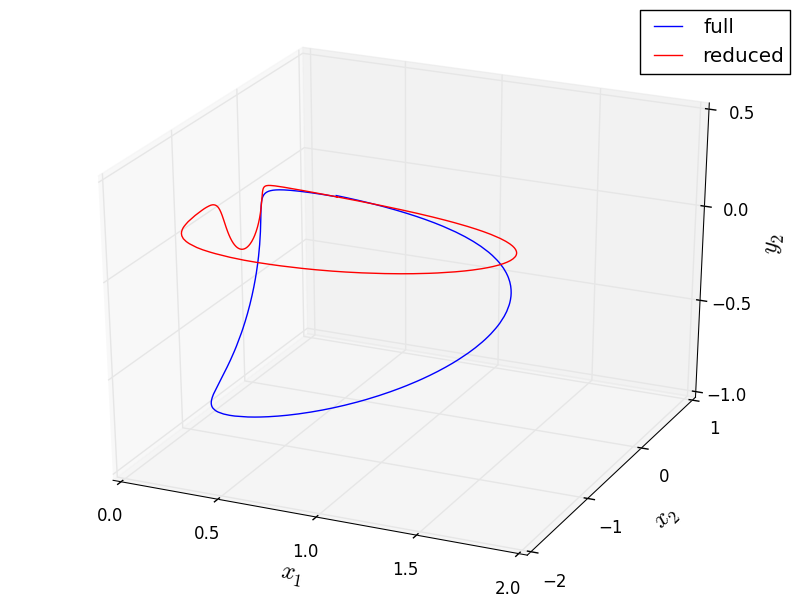
\includegraphics[width=0.8\textwidth]{twomodes_configuration}
  \caption[A \rpo\ in the \twomode\ system.]
  {
    The configuration of $\cycle{1}$ in the full \statesp\ projected
    into subspace $[x_{1},x_{2},y_{2}]$ (the blue curve) and in the slice (
    the red curve).
  }
  \label{fig:twomodes_configuration}
\end{figure}
In this subsection, we focus on one \rpo\ in the \twomode\ system
whose initial condition is
\begin{equation}
  \label{eq:2modeInit1}
  \cycle{1}: \quad (0.4525719,\quad 0.0,\quad 0.0509257,\quad 0.0335428)
  \,.
\end{equation}
The orbit has period $3.6415$.
\refFig{fig:twomodes_configuration} depicts \rpo\
$\cycle{1}$ in the full \statesp\ and in the slice.
The Floquet multipliers associated with this orbit are
\begin{equation}
  \label{eq:2modeMulti1}
  \ExpaEig_{j} : \quad (-1.481177, \quad
  -1.066888\cdot 10^{-09},\quad  0.999414,\quad  0.999913)
  \,.
\end{equation}
It has a weak expanding direction, a strong
contracting direction, and two marginal directions.

\begin{figure}[h]
  \centering
  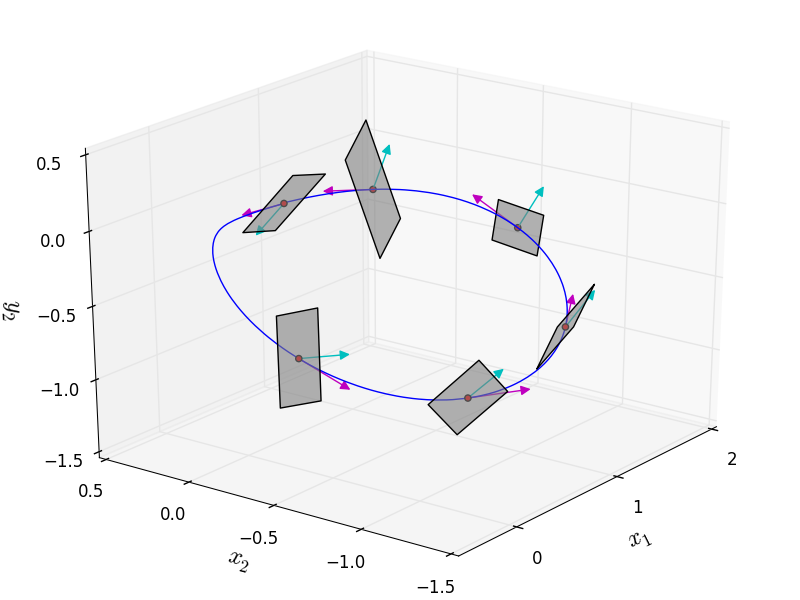
\includegraphics[width=0.8\textwidth]{twomodes_full}
  \caption[Marginal \Fv s in the \twomode\ system.]{
    The gray planes are spanned by the two marginal \Fv s.
    of \rpo\ $\cycle{1}$.
    The pink, green arrows are the velocity vectors and the group
    tangents on this orbit respectively.
    The blue curve is \rpo\ $\cycle{1}$ projected into the
    subspace $[x_{1},x_{2},y_{2}]$.
  }
  \label{fig:twomodes_full}
\end{figure}
The velocity field $\vel(\ssp)$ and the group tangent $\groupTan(\ssp)$
are \Fv s of this system and give rise to the two
marginal multipliers in \refeq{eq:2modeMulti1}, but the corresponding
two \Fv s are degenerate which cannot be told apart when we solving the
eigenequation of the \JacobianM. However, we can check whether $\vel(\ssp)$
and $\groupTan(\ssp)$ are contained in the subspace spanned by
these two \Fv s. This is the idea of \reffig{fig:twomodes_full},
in which we show the planes spanned by the two marginal \Fv s, the velocity field,
and the group tangent, along this orbit.
As we can see, $\vel(\ssp)$ and $\groupTan(\ssp)$ do lie in the planes.
Therefore, the calculation of Floquet spectrum and \Fv s
of $\cycle{1}$ is accurate at least for illustration purpose.

\begin{figure}[h]
  \centering
  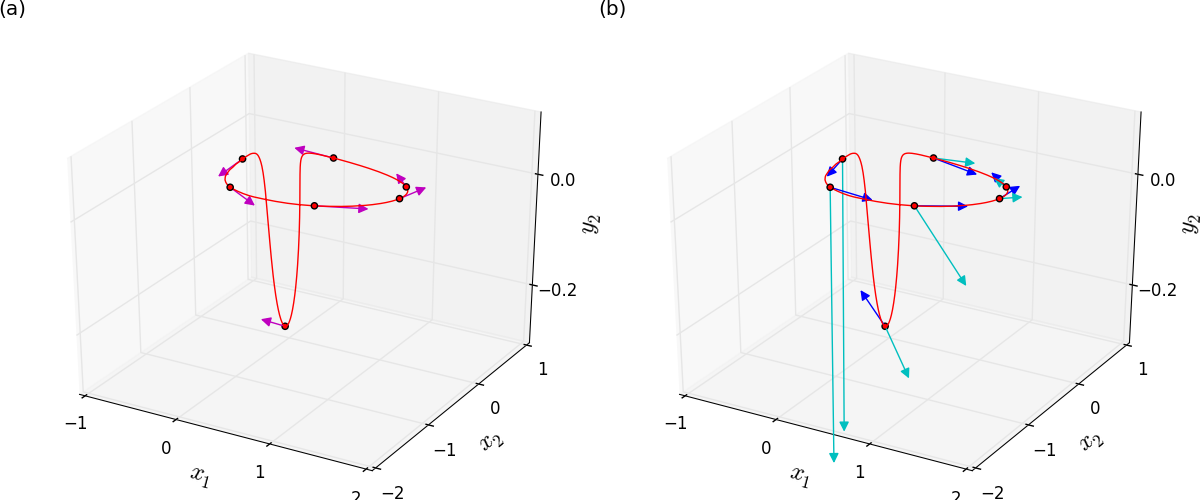
\includegraphics[width=1\textwidth]{twomodes_reduced}
  \caption[\Fv s in the slice in the \twomode\ system]{
    In-slice \Fv s for \rpo\ $\cycle{1}$.
    The red closed curve is $\cycle{1}$.
    (a) The marginal \Fv\ (pink).
    (b) The expanding (blue) and contracting (green) \Fv s in the slice.
  }
  \label{fig:twomodes_reduced}
\end{figure}

Now the task is to transform these \Fv s into the slice.
By the Lie group generator \refeq{2modefLieGen}, we get the
group tangent of an in-slice point
$\sspRed = \transp{(\hat{x}_1, 0, \hat{x}_2, \hat{y}_2)}$:
\[
  t(\sspRed)=(0,-\hat{x}_{1},2\hat{y}_{2},-2\hat{x}_{2})
  \,.
\]
Then by \refeq{projFullToSlice} we have
\[
  \pMat(\sspRed)=
  \begin{pmatrix}
    1 & 0 & 0 & 0 \\
    0 & 0 & 0 & 0 \\
    0 & 2\hat{y}_{1}/\hat{x}_{1} & 1 & 0 \\
    0 & -2\hat{x}_{2}/\hat{x}_{1} & 0 & 1 \\
  \end{pmatrix}
  \,.
\]
We choose to eliminate the second coordinate $\hat{y}_{1}$, then
\[
  \pMatM(\sspRed)=
  \begin{pmatrix}
    1 & 0 & 0 & 0 \\
    0 & 2\hat{y}_{1}/\hat{x}_{1} & 1 & 0 \\
    0 & -2\hat{x}_{2}/\hat{x}_{1} & 0 & 1 \\
  \end{pmatrix}
\,.
\]
Matrix $\pMatM(\sspRed)$ transforms \Fv s in the full \statesp\ into the
slice which are shown in \reffig{fig:twomodes_reduced}.
The group tangent $\groupTan(\sspRed)$, as one marginal vector,
disappears and the planes in \reffig{fig:twomodes_full}
collapse to the velocity
field along the orbit shown in \reffig{fig:twomodes_reduced}(a).
The other two projected \Fv s are shown in
\reffig{fig:twomodes_reduced}(b).

\begin{figure}[h]
  \centering
  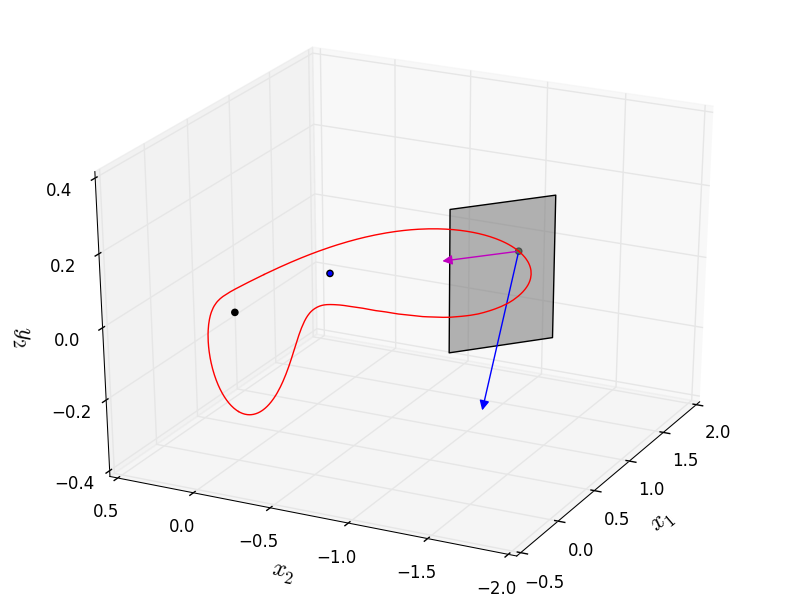
\includegraphics[width=0.8\textwidth]{twomodes_poincare}
  \caption[\Fv s on the {\PoincSec} in the \twomode\ system]{
    A vertical {\PoincSec} is constructed from the origin
    (black point) and a relative equilibrium
    (blue point) in
    the slice.
    The \PoincSec\ intersects $\cycle{1}$ (the red closed curve)
    at the green point.
    In-slice \Fv s are projected into the
    {\PoincSec}. The red/blue vector is the expanding/contracting
    \Fv. The marginal vector along the orbit disappears on the {\PoincSec}.
  }
  \label{fig:twomodes_poincare}
\end{figure}

In a similar way\rf{DasBuch}, \Fv s on
the slice could be
projected onto a {\PoincSec}. The projection matrix is
\[
  h_{\mathcal{P}}(\sspRed) = \matId -
  \frac{\ket{\hat{\vel}}\bra{\partial U}}{\braket{\hat{\vel}}{\partial U}}
  \,,
\]
where $U(x) = 0$ defines the {\PoincSec} with $\partial U$ its normal direction.
$\hat{\vel}$ is the in-slice velocity.
A \PoincSec\ can be fixed by choosing three points on it, or equivalently,
by three conditions. Here, we choose a ``vertical'' \PoincSec, namely, we demand
that the
$\hat{y}_2$ component of its normal direction vanishes. Next, this \PoincSec\
goes through the origin $(0,0,0)$ and a \reqv\
\[
  (\hat{x}_{e1}, \hat{x}_{e2},
  \hat{y}_{e2})=(0.439965,\quad -0.386267, \quad 0.070204)
  \,,
\]
shown in \reffig{fig:twomodes_poincare}.
In this case, $\partial U=(\hat{x}_{e2},- \hat{x}_{e1}, 0)$ and we get
\[
  h_{\mathcal{P}}(\sspRed)
  =\frac{1}{\hat{v}_{1}\hat{x}_{e2}-\hat{v}_{2}\hat{x}_{e1}}
  \begin{pmatrix}
    -\hat{v}_{2}\hat{x}_{e1} & \hat{v}_{1}\hat{x}_{e1} & 0 \\
    -\hat{v}_{2}\hat{x}_{e2} & \hat{v}_{1}\hat{x}_{e2} & 0 \\
    -\hat{v}_{3}\hat{x}_{e1} & \hat{v}_{3}\hat{x}_{e1} &
    \hat{v}_{1}\hat{x}_{e2}-\hat{v}_{2}\hat{x}_{e1}\\
  \end{pmatrix}
  \,.
\]
\refFig{fig:twomodes_poincare} shows the projected
expanding and contracting \Fv s
on the {\PoincSec}. The marginal vector (velocity field)
disappears.

\begin{figure}[h]
  \centering
  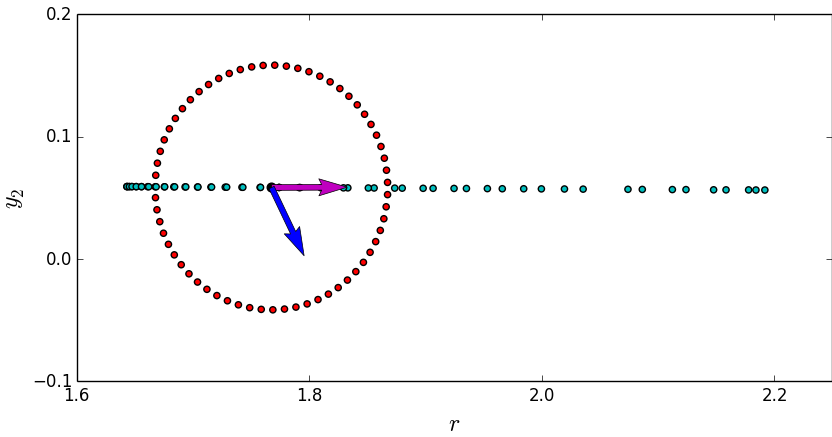
\includegraphics[width=0.8\textwidth]{twomodes_poincare_return}
  \caption[First returning points on the {\PoincSec} in
  the \twomode\ system]{
    A set of circularly (radis=0.1) distributed points (red)
    around the intersection
    point evolves for one period.
    Their first returning points (green) are recorded.
    The pink and blue arrows are the expanding
    and contracting
    \Fv s projected onto the {\PoincSec} respectively.
    Here $r=(\hat{x}_{1}^2+\hat{x}_{2}^2)^{1/2}$.
  }
  \label{fig:twomodes_poincare_return}
\end{figure}

Last, \reffig{fig:twomodes_poincare_return} shows the
{\PoincSec} and the
two projected \Fv s. A set of
circularly distributed points around
the intersection point  evolves for one period
and their first returning points are
recorded.
The contracting direction is close to the vertical direction,
and \refeq{eq:2modeMulti1} says that the contracting rate is large
in this direction. Therefore,
the returning points are squashed heavily in the
vertical direction; however, the magnitude of expanding multiplier is
about 1.5, so the elongation in the horizontal direction is relatively
small.

In summary,
we have reduced the \SOn{2} symmetry of the \twomode\ system
and discussed the \Fv s of a specific \rpo\ in the full state space and in the
slice. The marginal direction along the group orbit tangent is eliminated by the
slice. Furthermore, we have constructed a \PoincSec\ of codimension two with
respect to the original system. In this \PoincSec, the \rpo\ $\cycle{1}$
is reduced to a fixed point with
one expanding and one contracting \Fv, and the dynamics is
greatly simplified. This simple example illustrates why symmetry reduction
is an indispensable tool when studying dynamical systems with
continuous symmetries.

